\refstepcounter{section}
\section*{Lecture 12: Landau Theory for Phase Transition: II}
\addcontentsline{toc}{section}{Lecture 12: Landau Theory for Phase Transition: II}
We now add a cubic term to the free energy, which will lead to a first order transition.
\subsection{First Order Transition}
\begin{equation}
    \SL= \frac{1}{2}a_2(T-T_c) m^2-\frac{1}{3}a_3m^3+\frac{1}{4}a_4m^4 \qquad a_4, a_2>0
\end{equation}
We can assume the $a_3>0$, if not, define $m'=-m$. The free energy no longer enjoys the $\inte_2$ symmetry. Minimising the free energy gives us,
\begin{align*}
    \pdv{\SL}{m} = a_2(T-T_c)m - a_3m^2 + a_4m^3 =0 \implies m=0 \quad \text{or}\quad   a_4m^2-a_3m +a_2(T-T_c)=0
\end{align*}
The quadratic part gives us two solutions, namely, 
$$m_\pm = \frac{a_3}{2a_4}\pm \sqrt{\qty(\frac{a_3}{2a_4})^2 - \frac{a_2}{a_4}(T-T_c)}$$
From this, we see that if $a_3^2<4a_2a_4(T-T_c)$ then the above two solutions become complex and we are left with only $m=0$ as the real solution. If $a_3^2>4a_2a_4(T-T_c)\implies T<T_c+\frac{a_3^2}{4a_2a_4}$, then we have three real solutions. Let us denote $T^* = T_c+\frac{a_3^2}{4a_2 a_4}>T_c$, which implies that even above $T_c$, for $T$ satisfying $T_c<T<T^*$, three solutions do appear.\\[0.2cm]
Okay, now let us see the position of these three extremas. Note that $m_+>m_-$ and $m_+>0$ from the form of the expression, so only the position with respect to zero needs to be ascertained for $m_-$. If we want $m_->0$, then 
\begin{align*}
    \qty(\frac{a_3}{2a_4})^2 >\qty(\frac{a_3}{2a_4})^2 - \frac{a_2}{a_4}(T-T_c) \implies T>T_c
\end{align*}
Thus, for $T>T_c$ we have $m_+>m_->0$ and for $T<T_c$ we have $m_-<0<m_+$. The position of the extremas are fixed. Now, let's look at the curvature.
\begin{align*}
    \pdv[2]{\SL}{m} = a_2(T-T_c) - 2a_3m+3a_4m^2 
\end{align*}
At $m=0$, $\pdv[2]{\SL}{m}  = a_2(T-T_c)$ which implies that for $T<T_c$ we have a maxima at $m=0$ and for $T>T_c$, there's a minima at $m=0$. From these facts, we have: 
\begin{itemize}
    \item For $T<T_c$, $m_\pm$ are the minima and $m=0$ is the maxima.
    \item For $T>T_c$, $m_+$ and $m=0$ are the minima and $m_-$ is the maxima.
\end{itemize}
 Let us now see how the free energy behaves for different values of $T>T_c$, to ascertain which extremas are global. At $m=0$, we always have an minima and hence, to find the global things, we neet to compare the other extremas with $\SL(m=0)$, so we look at the case when $\SL(0) = \SL(m_{+})$ (since $m_-$ is the maxima, we do not care about it). This is equivalent to simultaneously satisfying the two equations for $m\neq 0$, 
 \begin{equation*}
    \SL(m) = 0 \qquad \pdv{\SL}{m} = 0 
 \end{equation*}
 Eliminating $m^2$ from these equations and definining $\epsilon = T-T_c$, leaves us with,
 $$4\qty(\frac{1}{3}a_3 m - \frac{1}{2}a_2\epsilon) - a_3m + a_2\epsilon = 0$$
 from which we get, $m = \frac{3a_2\epsilon}{a_3}$. Now, this $m$ must be equal to $m_+$, since this is the minima.
 \begin{align*}
    \implies& \qty(\frac{3a_2}{a_3}\epsilon -\frac{a_3}{2a_4})^2 = \qty(\frac{a_3}{2a_4})^2 - \frac{a_2}{a_4}\epsilon\\
    \implies& \qty(\frac{3a_2}{a_3})^2\epsilon^2 - \frac{3a_2}{a_4}\epsilon = -\frac{a_2}{a_4}\epsilon \\
    \implies&\frac{9a_2}{a_3^2\epsilon} = \frac{2}{a_4}\\
    \implies& \boxed{a_3^2 = \frac{9}{2}a_2a_4\epsilon}
 \end{align*}
 Define $T^{**} =T_c+ \frac{2a_3^2}{9a_2a_4}<T^*$. We summarise all the cases below:
 \begin{itemize}
    \item For $T>T^*$ we have only one minima $m=0$.
    \item For $T^{**}<T<T^*$ we have three extrema, the global minima is at $m=0$ and at $m_+$ we have a local minima. $m_-$ is a maxima.
    \item For $T_c<T<T^{**}$ we have three extrema, the global minima is at $m_+$ and at $m=0$ we have a local minima.  $m_-$ is still a maxima.
    \item For $T<T_c$, we have three extremas and $m=0$ is a local maxima, while the global minima is at $m_+$.  $m_-$ is a local minima.
 \end{itemize}
 \begin{figure}[t]
    \centering
    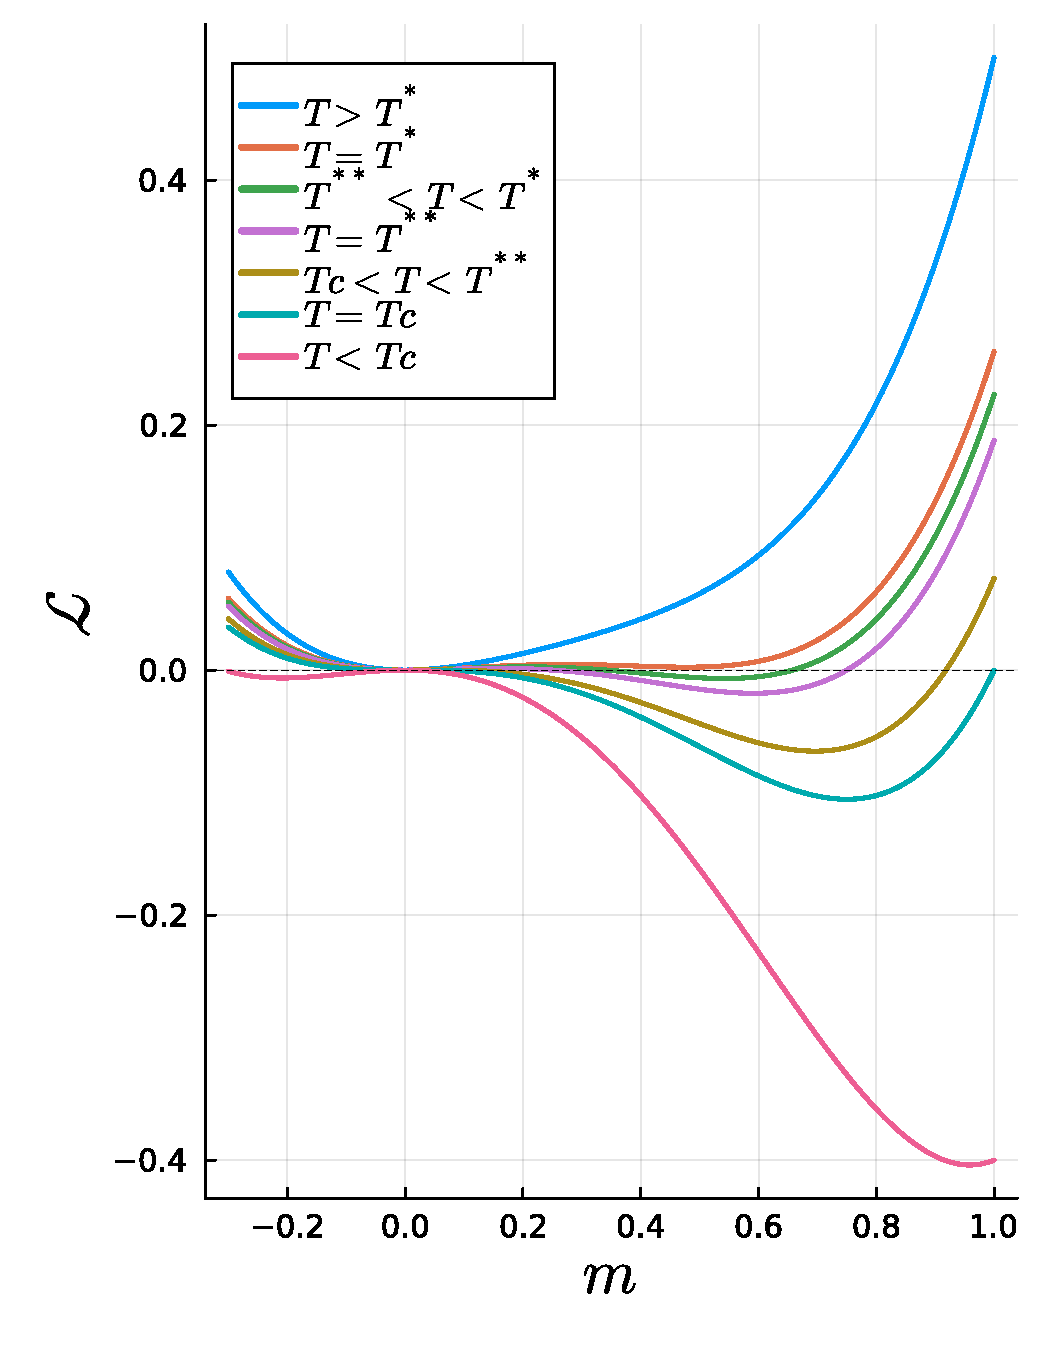
\includegraphics[scale=0.5]{codes/first_order.pdf}
    \caption{Landay free energy $\SL$ with the cubic term, for different values of temperature.}
 \end{figure}
\subsection{Tricritical Point}
